\section{BASE TEÓRICA}
\subsection{Máquina de Estados Finitos (FSM)}
\sangria{} En lógica digital, una máquina de estados finitos es un sistema secuencial sincrónico cuyo comportamiento depende tanto de las entradas actuales como de su historial pasado. Se compone formalmente de tres bloques principales:
\begin{itemize}[nosep]
	\item \textbf{Registro de estado (memoria):} es un conjunto de flip-flops sincronizados por un reloj (CLK) que almacenan el estado actual ($Q(t)$).
	\item \textbf{Lógica combinacional de estado siguiente:} red de compuertas que calcula el estado futuro ($Q(t+1)$) a partir del estado actual y las entradas externas.
	\item \textbf{Lógica combinacional de salida:} red que genera las salidas externas del circuito.
\end{itemize}
\hspace{5pt}
\sangria{} A partir de aquí se desprenden dos máquinas: la de Moore y una de Mealy, la diferencia radica en cómo se calcula la lógica combinacional de salida.
\subsubsection{Máquina de Moore}
\sangria{} Las salidas externas del sistema son función única y exclusivamente del estado actual de los flip-flops.
{\Large
\[
	Salida_{Moore} = f(Q(t))
\]
}
\begin{itemize}[nosep]
	\item\textbf{Sincronización:} dado a que la salida depende solo de los valores almacenados en los flip flops (que solo cambian en los flancos activos del reloj), la salida está perfectamente sincronizada con el reloj.
	\item\textbf{Estabilidad y seguridad:} es un modelo más estable y libre de picos falsos o valores transitorios (glitches) generados por las variaciones en las entradas.
	\item\textbf{Representación en diagramas:} la salida se describe dentro del círculo/nodo del estado junto al nombre o código del estado (ejemplo: $S_0/Z = 0$).
	\item\textbf{Cantidad de estados:} generalmente requiere más estados, por ende son más flip flops, para resolver una tarea.
\end{itemize}

\subsubsection{Máquina de Mealy}
\sangria{} Las salidas externas son función tanto del estado actual como el de las entradas externas actuales.
{\Large 
\[
	Salida_{Mealy} = f(Q(t), X)
\] 
}

\begin{itemize}[nosep]
	\item\textbf{Respuesta inmediata:} existe un acoplamiento directo entre la salida y la entrada, lo que permite que el sistema reaccione instantáneamente ante un cambio en las entradas sin tener que esperar al siguiente flanco de reloj.
	\item\textbf{Comportamiento temporal:} si las entradas cambian en medio de un ciclo de reloj, la salida puede cambiar o presentar glitches (valores transitorios erróneos). Para evitarlos, las salidas en Mealy deben muestrearse con cuidado o sincronizarse externamente.
	\item\textbf{Representación en diagramas:} las salidas no se ubican dentro de los estados, sino sobre flechas de transición con la sintaxis $Entrada/Salida$.
	\item\textbf{Cantidad de estados:} al ''externalizar'' la lógica de salida hacia las transiciones, suele requerir menos estados que la versión de Moore para el mismo problema.
\end{itemize}

\section{DESARROLLO}
\usetikzlibrary{shapes.geometric, arrows.meta, positioning}

\tikzstyle{block} = [rectangle, rounded corners, align=center,minimum width=1cm, minimum height=1cm,
text centered, draw=black, fill=gray!10]
\tikzstyle{arrow} = [thick, -{Stealth[length=3mm]}]
\begin{center}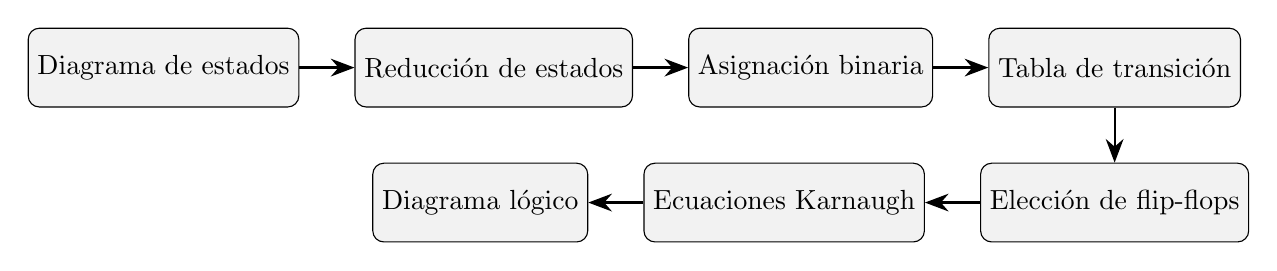
\begin{tikzpicture}[node distance=0.7cm]

\node (2) [block] {Diagrama de estados};
\node (3) [block, right=of 2] {Reducción de estados};
\node (4) [block, right=of 3] {Asignación binaria};
\node (5) [block, right=of 4] {Tabla de transición};
\node (6) [block, below=of 5] {Elección de flip-flops};
\node (7) [block, left=of 6] {Ecuaciones Karnaugh};
\node (8) [block, left=of 7] {Diagrama lógico};
%\node (3) [block, right=of 2] {Cerrar el interruptor $S_w$};
%\node (4) [block, below=of 3] {Variar el potenciómetro para relevar las tensiones $V_G$};
%\node (5) [block, right=of 4] {Graficar los valores obtenidos \\y comparar la curva $I_G = f(V_G)$};
%\node (6) [block, below=of 5] {Colocar $V_G = 0$ V y cerrar el switch};
%\node (7) [block, left=of 6] {Colocar $V_{CC} = 100$ V};
%\node (8) [block, below=of 7] {Subir lentamente $V_G$ hasta observar un cambio importante\\ en $I_{AK}$ (disparo del SCR). Anotar $V_G$ e $I_G$.};
%\node (9) [block, below=of 8] {Manteniendo el potenciómetro en esa posición, \\abrir $S_w$ y analizar el comportamiento de $I_{AK}$.};
%\node (10) [block, below=of 9] {Con $S_w$ abierto, bajar $V_{CC}$ en pasos de 10 V \\(y de 1 V en los últimos 10 V), registrando $I_{AK}$.};
%\node (11) [block, right=of 10] {Subir nuevamente $V_{CC}$ hasta \\ 100 V y observar el \\comportamiento de $I_{AK}$.};
%\node (12) [block, below=of 11] {Cerrar $S_w$ corroborando \\que $V_G$ e $I_G$ \\sean los mismos valores\\ relevados antes.};
%\node (13) [block, left=of 12] {Analizar qué sucedió con $I_{AK}$ cuando se cerró el interruptor.};
%\node (14) [block, below=of 13] {Abrir nuevamente $S_w$ y observar $I_{AK}$.};
%\node (15) [block, below=of 14] {Desconectar las tensiones de alimentación sin mover el potenciómetro, e invertir Ánodo y Cátodo del SCR.};
%\node (16) [block, below=of 15] {Reconectar las alimentaciones y cerrar $S_w$. Analizar el comportamiento de $I_{AK}$.};

\foreach \i [evaluate=\i as \j using int(\i+1)] in {2,...,7}
    \draw [arrow] (\i) -- (\j);

\end{tikzpicture}
\end{center}

\subsection{En máquina de Moore}
\subsubsection{Mapeo de entradas y salidas}
\sangria{} Identificando el montacargas, se obtiene:\\[5pt]
\begin{itemize}[nosep]
	\item $S_1$: final de carrera piso 1 (sensor).
	\item $S_2$: final de carrera piso 2 (sensor).
	\item $L$  : es el botón de llamada.
	\item $MS$ : activa el motor para ascender el montacargas.
	\item $MB$ : activa el motor para descender el montacargas.
\end{itemize}
\sangria{} Las entradas al sistema serán nuestros sensores y el botón de llamada, en tanto que las salidas del sistema serán las órdenes para ascender o descender el montacargas por medio del motor. Tanto los sensores de entrada y las salidas usarán ''1'' para indicar una señal viva.
\subsubsection{Los estados de Moore}
\sangria{} El modelo de Moore depende exclusivamente del estado actual, por lo que no se podría representar en un solo estado por ejemplo ''estar en el piso 1'' si desde allí el motor tiene que encenderse o apagarse, que sería otro estado más. Se debería implementar un diseño para los estados en reposo y los estados en movimiento:\\[5pt]
\begin{enumerate}[nosep] 
	\item $S_0$ REPOSO EN PISO 1 $\rightarrow$ $MS$ y $MB$ son 0.
	\item $S_1$ SUBIENDO	$\rightarrow$ $MS$ = 1 y $MB$ = 0.
	\item $S_2$ REPOSO EN PISO 2 $\rightarrow$ $MS$ y $MB$ son 0.
	\item $S_3$ BAJANDO $\rightarrow$ $MS$ = 0 y $MB$ = 1.
\end{enumerate}
\subsubsection{Asignación binaria}
\sangria{} Al tener $N=4$ estados, aplicamos:
\[
	N \leq 2^n
\]

siendo $n$ la cantidad de flip flops, por lo tanto: 
\[
	log(N) = n\cdot{}log(2),\qquad{}\text{Logaritmo ambos miembros}
\]
\[
	\frac{log(N)}{log(2)} = n,\qquad{}\text{Multiplicar ambos miembros por log(2)}
\]
\[
	log_2(N) = n,\qquad{}\text{Propiedad cociente de logaritmos de igual base}
\] 
\[
	\Rightarrow log_2(4) = n,\qquad{}\text{Reemplazar y evaluar}
\]
\[
	n = 2
\]
\begin{center}CANTIDAD DE FLIP FLOPS=2 ($Q_1$,$Q_0$) \end{center}
\sangria{} Se asigna combinaciones binarias para cada estado:
\begin{itemize}[nosep]
	\item Reposo P1($S_0$): $Q_1Q_0 = 00$
	\item Subiendo ($S_1$): $Q_1Q_0 = 01$
	\item Reposo P2 ($S_2$): $Q_1Q_0 = 10$
	\item Bajando ($S_3$): $Q_1Q_0 = 11$
\end{itemize}
\subsubsection{Tabla de transiciones}
\begin{center}
\centering
\definecolor{evenrow}{HTML}{C0C0C0}
\rowcolors{2}{}{evenrow}
\begin{tabular}{cc|ccc|cc|cc|cc}
\cline{1-9}
\rowcolor[HTML]{656565} 
\multicolumn{2}{c|}{\cellcolor[HTML]{656565}{\color[HTML]{FFFFFF} \textbf{ESTADO ACTUAL}}} & \multicolumn{3}{c|}{\cellcolor[HTML]{656565}{\color[HTML]{FFFFFF} \textbf{ENTRADAS}}} & \multicolumn{2}{c|}{\cellcolor[HTML]{656565}{\color[HTML]{FFFFFF} \textbf{ESTADO SIGUIENTE}}} & \multicolumn{2}{c|}{\cellcolor[HTML]{656565}{\color[HTML]{FFFFFF} \textbf{SALIDAS}}} & \multicolumn{2}{c}{\cellcolor[HTML]{656565}{\color[HTML]{FFFFFF} \textbf{SECUENCIA ESTADO}}} \\ \hline
$Q_1$                                        & $Q_0$                                       & $S_1$                       & $S_2$                       & $L$                       & $Q_1(t+1)$                                    & $Q_0(t+1)$                                    & $MS$                                      & $MB$                                     & $S_n$ (Leer $Q_1Q_0$)                  & Lectura                                             \\
0                                            & 0                                           & 0                           & 0                           & 0                         & 0                                             & 0                                             & 0                                         & 0                                        & 00 -\textgreater{} 00                  & Reposo P1 -\textgreater{} Reposo P1                 \\
0                                            & 0                                           & 0                           & 0                           & 1                         & 0                                             & 1                                             & 0                                         & 0                                        & 00 -\textgreater{} 01                  & Reposo P1 -\textgreater{} Subiendo                  \\
0                                            & 0                                           & 1                           & x                           & x                         & 1                                             & 1                                             & 0                                         & 0                                        & 00 -\textgreater{} 11                  & Reposo P1 -\textgreater{} Bajando                   \\
0                                            & 1                                           & x                           & x                           & x                         & 1                                             & 0                                             & 1                                         & 0                                        & 01 -\textgreater{} 10                  & Subiendo -\textgreater{} Reposo P2                  \\
1                                            & 0                                           & 0                           & 0                           & 0                         & 1                                             & 0                                             & 0                                         & 0                                        & 10 -\textgreater{} 10                  & Reposo P2 -\textgreater{} Reposo P2                 \\
1                                            & 0                                           & 0                           & 0                           & 1                         & 1                                             & 1                                             & 0                                         & 0                                        & 10 -\textgreater{} 11                  & Reposo P2 -\textgreater{} Bajando                   \\
1                                            & 0                                           & x                           & 1                           & x                         & 0                                             & 1                                             & 0                                         & 0                                        & 10 -\textgreater{} 01                  & Reposo P2 -\textgreater{} Subiendo                  \\
1                                            & 1                                           & x                           & x                           & x                         & 0                                             & 0                                             & 0                                         & 1                                        & 11 -\textgreater{} 00                  & Bajando -\textgreater{} Reposo P1                  
\end{tabular}
\end{center}
\subsubsection{Elección de flip flops}
\sangria{} Se usará flip flops D. Como se denota: la entrada de datos es directamente el estado futuro. Los motivos de su elección es por barato de conseguir y por ser el más directo: si se necesita que el próximo estado sea un 1, se introduce un 1 en la entrada D; mismo caso con un 0. El paso de la tabla de transición a los mapas de karnaugh es más directo.
\imagen[]{5cm}{./imagenes/flipflopD.png}
\begin{center}
\centering
\begin{tabular}{|c|c|}
\hline
\rowcolor[HTML]{656565} 
{\color[HTML]{FFFFFF} \textbf{$Q(t+1)$}} & {\color[HTML]{FFFFFF} \textbf{$D$}} \\ \hline
0                                        & 0                                   \\ \hline
1                                        & 1                                   \\ \hline
\end{tabular}
\end{center}
\subsubsection{Reducción de ecuaciones}
\sangria{} Las variables son:
\begin{itemize}[nosep] 
	\item 2 para el estado actual: $Q_1Q_0$
	\item 3 para las entradas externas: $S_1,S_2$ y $L$
\end{itemize}
Esto significa que cada uno de los mapas de karnaugh debe ser de 5 variables. Como un mapa de 5 variables es igual a dos mapas de 4 variables superpuestos, suele ser más cómodo dividirlos usando una de las variables para separar los mapas: para $L = 0$ y otro para $L = 1$. Para $D_1$ el estado futuro es $Q_1(t+1)$

\midTitle{Black}{Para $D_1$ con $L=0$}{}\\[5pt]
Mirando la tabla de transiciones, tenemos que:
\begin{itemize}[nosep]
	\item $<Q_1;Q_0;S_1;S_2>\qquad{} =\qquad{} <0;0;0;0> \qquad{}\rightarrow \qquad{} Q_1(t+1) = 0$ 
	\item $<Q_1;Q_0;S_1;S_2>\qquad{} =\qquad{} <0;0;0;0> \qquad{}\rightarrow \qquad{} Q_1(t+1) = 0$. Pero acá $L=1$ y estamos analizando $L=0$, no lo contamos.
	\item $<Q_1;Q_0;S_1;S_2>\qquad{} =\qquad{} <0;0;1;x> \qquad{}\rightarrow \qquad{} Q_1(t+1) = 1$ 
	\item $<Q_1;Q_0;S_1;S_2>\qquad{} =\qquad{} <0;1;x;x> \qquad{}\rightarrow \qquad{} Q_1(t+1) = 1$ 
	\item $<Q_1;Q_0;S_1;S_2>\qquad{} =\qquad{} <1;0;0;0> \qquad{}\rightarrow \qquad{} Q_1(t+1) = 1$ 
	\item $<Q_1;Q_0;S_1;S_2>\qquad{} =\qquad{} <1;0;0;0> \qquad{}\rightarrow \qquad{} Q_1(t+1) = 1$. Pero $L=1$, no va.
	\item $<Q_1;Q_0;S_1;S_2>\qquad{} =\qquad{} <1;0;x;1> \qquad{}\rightarrow \qquad{} Q_1(t+1) = 0$ 
	\item $<Q_1;Q_0;S_1;S_2>\qquad{} =\qquad{} <1;1;x;1> \qquad{}\rightarrow \qquad{} Q_1(t+1) = 0$ 
\end{itemize}
Analizando para $Q_1Q_0 = 00$:
\begin{itemize}[nosep]
	\item $S_1S_2 = 00$ el estado siguiente es $Q_1(t+1) = 1$
	\item $S_1S_2 = 1X$ como $S_2 = X$ y $L=X$, aplico que $L=0$ (don't care) y $S_2$ puede ser 1 o 0. Para el mapa, con $S_2 = X$, $Q_1(t+1)$ vale 1. 
	\item $S_1S_2 = 01$ esta combinación no existe en la tabla, vale $X$.
\end{itemize}
Analizando para $Q_1Q_0 = 01$:
\begin{itemize}[nosep]
	\item $S_1S_2= XX$, no importa el estado de los sensores, $Q_1(t+1) = 1$. Esta columna tiene todo en 1.
\end{itemize}
Analizando para $Q_1Q_0 = 11$:
\begin{itemize}[nosep]
	\item El estado de los sensores es $X$ con $Q_1(t+1) = 0$. Toda la columna tiene 0.
\end{itemize}
Analizando para $Q_1Q_0 = 10$:
\begin{itemize}[nosep]
	\item $S_1S_2$ valen 0 y $Q_1(t+1) = 1$.
\end{itemize}
\begin{center}
	\begin{karnaugh-map}[4][4][1][$Q_1Q_0$][$S_1S_2$]
		% Q_1Q_0 = 00
		\minterms{8,12}
		\maxterms{0}
		\terms{4}{X}
		% Q_1Q_0 = 01
		\minterms{1,5,13,9}
		% Q_1Q_0 = 11
		\maxterms{3,7,15,11}
		% Q_1Q_0 = 10
		\minterms{2}
		\maxterms{6,14}
		\terms{10}{X}
		\implicantedge{2}{2}{10}{10}
		\implicant{1}{9}
		\implicant{12}{9}
	\end{karnaugh-map}
\end{center}
\midTitle{Black}{Para $D_1$ con $L=1$}{}
\begin{center}
	\begin{karnaugh-map}[4][4][1][$Q_1Q_0$][$S_1S_2$]
		%Q_1Q_0 = 00
		\maxterms{0}
		\minterms{12,8}
		\terms{4}{X}
		%Q_1Q_0 = 01
		\minterms{1,5,13,9}
		%Q_1Q_0 = 11
		\maxterms{3,7,15,11}
		%Q_1Q_0 = 10
		\minterms{2}
		\maxterms{6,14}
		\terms{10}{X}

		\implicantedge{2}{2}{10}{10}
		\implicant{1}{9}
		\implicant{12}{9}
	\end{karnaugh-map}
\end{center}
\midTitle{Black}{$D_0 = Q_0(t+1)$ con $L=0$}{}
\begin{center}
	\begin{karnaugh-map}[4][4][1][$Q_1Q_0$][$S_1S_2$]
		%Q_1Q_0 = 00
		\maxterms{0}
		\minterms{12,8}
		\terms{4}{X}
		%Q_1Q_0 = 01
		\maxterms{1,5,13,9}
		%Q_1Q_0 = 11
		\maxterms{3,7,15,11}
		%Q_1Q_0 = 10
		\maxterms{2}
		\minterms{6,14}
		\terms{10}{X}

		\implicant{12}{8}
		\implicantedge{4}{12}{6}{14}
	\end{karnaugh-map}
\end{center}
\midTitle{Black}{$D_0 = Q_0(t+1)$ con $L=1$}{}
\begin{center}
	\begin{karnaugh-map}[4][4][1][$Q_1Q_0$][$S_1S_2$]
		%Q_1Q_0 = 00
		\minterms{0,12,8}
		\terms{4}{X}
		%Q_1Q_0 = 01
		\maxterms{1,5,13,9}
		%Q_1Q_0 = 11
		\maxterms{3,7,15,11}
		%Q_1Q_0 = 10
		\minterms{2,6,14}
		\terms{10}{X}

		\implicantedge{0}{8}{2}{10}
	\end{karnaugh-map}
\end{center}
\midTitle{Black}{Ecuaciones}{}
\[
	D_1 = \overline{L}\cdot{}\text{(Karnaugh de $D_1$ para $L=0$)} + L\cdot{}\text{(Karnaugh de $D_1$ para $L=1$)}
\]
\[
	D_1 = \overline{L}\cdot{}(Q_1\cdot\overline{Q_0}\cdot\overline{S_2} + \overline{Q_1}\cdot{}Q_0+S_1\cdot{}\overline{Q_1}) + L\cdot{}(\overline{S_2}\cdot\overline{Q_0}\cdot{}Q_1+\overline{Q_1}\cdot{}Q_0+S_1\cdot\overline{Q_1})
\]
\[
	D_1 = (Q_1\cdot\overline{Q_0}\cdot\overline{S_2} + \overline{Q_1}\cdot{}Q_0+S_1\cdot{}\overline{Q_1})\cdot{}(\overline{L}+L),\qquad{}\text{como}\quad\overline{L}+L=1
\]
\[
	\colorbox{yellow}{$D_1 = Q_1\cdot\overline{Q_0}\cdot\overline{S_2} + \overline{Q_1}\cdot{}Q_0+S_1\cdot{}\overline{Q_1}$}
\]


\[
	D_0 = \overline{L}\cdot{}\text{(Karnaugh de $D_0$ para $L=0$)} + L\cdot{}\text{(Karnaugh de $D_0$ para $L=1$)}
\]
\[
	D_0 = \overline{L}\cdot{}(S_2\cdot\overline{Q_0} + S_1\cdot\overline{Q_1}\cdot\overline{Q_0}) + L\cdot{}\overline{Q_0}
\]
\[
	\colorbox{yellow}{$D_0 = \overline{Q_0}\cdot{}[\overline{L}\cdot{}(S_2 + S_1\cdot\overline{Q_1})+L]$}
\]

\[
	\colorbox{yellow}{$MS = \overline{Q_1}\cdot{}Q_0$}
\]
\[
	\colorbox{yellow}{$MB = Q_1\cdot{}Q_0$}
\]

\subsubsection{Diagrama lógico}
\imagen[$D_1$ Moore]{15cm}{./imagenes/d1Moore.png}
